\documentclass[border=0.2cm,convert]{standalone}
\usepackage{tikz}

% xelatex --shell-escape *.tex
\usetikzlibrary{arrows,trees,positioning}

\tikzset{level distance=2em}
\tikzset{level 1/.style = {sibling distance = 5cm}}
\tikzset{level 2/.style = {sibling distance = 2.5cm}}
\tikzset{level 3/.style = {sibling distance = 1.5cm}}
\tikzset{level 4/.style = {sibling distance = 1cm}}
\tikzset{every node/.style={draw,circle}}

\tikzset{black/.style={circle, white, draw=black, fill=black, font=\bfseries\sffamily}}
\tikzset{red/.style={circle, draw=red, font=\bfseries\sffamily, very thick}}
\tikzset{nil/.style={rectangle, draw=black, very thick}}

\begin{document}
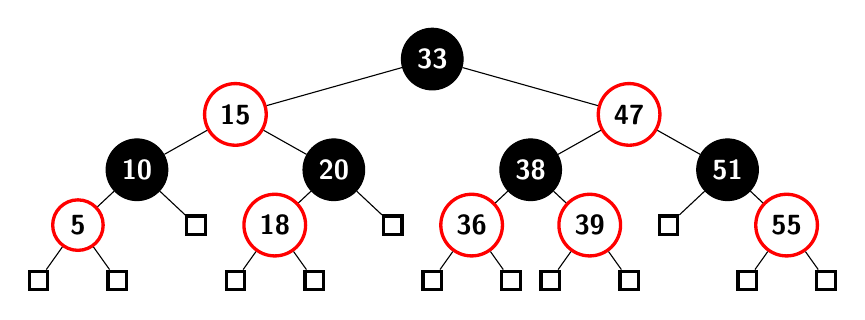
\begin{tikzpicture}
\node[black]{33}
    child {
        node[red]{15}
        child {
            node[black]{10}
            child {
                node[red]{5}
                child {node[nil]{}}
                child {node[nil]{}}
            }
            child {node[nil]{}}
        }
        child {
            node[black]{20}
            child {
                node[red]{18}
                child {node[nil]{}}
                child {node[nil]{}}
            }
            child {node[nil]{}}
        }
    }
    child {
        node[red]{47}
        child {
            node[black]{38}
            child {
                node[red]{36}
                child {node[nil]{}}
                child {node[nil]{}}
            }
            child {
                node[red]{39}
                child {node[nil]{}}
                child {node[nil]{}}
            }
        }
        child {
            node[black]{51}
            child {node[nil]{}}
            child {
                node[red]{55}
                child {node[nil]{}}
                child {node[nil]{}}
            }
        }
    };
\end{tikzpicture}
\end{document}
